\documentclass{JMLFS}

\journal{JMLFS-ID}%Letters in High Energy Physics}
\vol{2020}

%%\publishedtrue%%Uncomment to get following information on first page
\received{xx January 2018}
\published{xx March 2018}

\def\be{\begin{equation}}
\def\ee{\end{equation}}
\def\bea{\begin{eqnarray}}
\def\eea{\end{eqnarray}}
\def\met{\not{\!{\rm E}}_T}
\def\zp{Z^\prime}

\newcommand{\bi}{\bibitem}
\newcommand{\nn}{\nonumber}
\def\BibTeX{\rm B{\sc ib}\TeX}

\begin{document}

\title{Learning Concepts using Deep Neural Networks}

\author{Sunil Kumar Vengalil,\auno{1} Neelam Sinha\auno{2}  and G Srinivasaraghavan,\auno{3}}
\address{$^1$International Institute of Information Technology Bangalore}
\address{$^2$International Institute of Information Technology Bangalore}
\address{$^3$International Institute of Information Technology Bangalore}

\begin{abstract}
The ML revolution is in full swing. In fact, the groundwork for it was prepared in the middle of the 20th century, yet, it is only with the ever continuing development of increasingly powerful computers, combined with computational algorithms refined over the past couple of decades, that the world has seen an explosion of applications of ML, in anything from health, to finance down to even autonomous cars!
\end{abstract}

\maketitle

\begin{keyword}
Machine Learning\sep Artificial Intelligence\sep Computer Science
\doi{10.2018/JMLFS000001}
\end{keyword}

\section{Introduction}
With the advent of Deep learning in the past decade,  Machine Learning and Deep Learning models have changed their role from a "merely research idea" to an essential component in almost all domains ranging from Banking Finance and Insurance Sector(BFIS), retail, manufacturing to medical\cite{jordan2015} and healthcare.
However, one of the major pain points of deep learning models, when used in industry, is the lack of explainability, i.e., they are unable to provide the exact reason for prediction.
One the one hand, researchers build complex ensemble and deep architectures in order to increase the classification accuracy, which results in increased accuracy but the more complex the model is, the more difficult to provide explanations for the predictions.
This trade off between accuracy and explainability of Machine Learning and Deep Learning models is well known \cite{wu2021}.
In many use cases, like medical, customer churn prediction in Banking Finance and Insurance Sector(BFIS), fraud and spam detection etc, it is as equally important to get an explainable prediction as getting correct predictions.
An explainable prediction can be easily converted to action item.
Sometimes one might even want to compromise with a less accurate model, if it can provide better explanations for the predictions.
This behaviour of Machine Learning and Deep Learning models is in sharp contrast with how humans learn.

Learning in human posses the following special characteristics which the ML and DL models starve to achieve.
\begin{enumerate}

\item When humans learns something new, over a period of time they gradually  1)internalize the concepts 2) abstracts the concepts and 3) reuse the concepts in related tasks- all these accomplished usually from a very few samples \cite{lake2015}.

\item The learned concepts are more generic as opposed the predictions, they make using the concept, in a particular scenario.
Each scenario might be different, but the concept used to make an inference will be same.
In other words, they use the same concept to make predictions for different input scenarios i.e the mapping between concept and scenario is one to many.

\item Humans can always provide an explanation for what they predict using the concepts they learned (Irrespective of the fact that the prediction might be wrong).

\end{enumerate}
In this article, we explore how such behaviours can be incorporated into deep learning models.
Explainability in DL models is something which has been actively researched and many approaches has been suggested in the literature in last decade\cite{linardatos2021}.
See section \ref{lit_survey_explainability} for an extensive literature survey of explainability on deep learning models.
However, our objective in this article is not just to inject explainability into a trained deep learning model.
We rather, focus on how the underlying model can learn \textbf{generalized concepts}  which are used to make predictions.
There has been previous studies \cite{lake2015} on developing models that learn concepts and use the learned concepts in a human like manner using Bayesian Probabilistic Language \cite{tenenbaum2019}.

In this study, we report results of experiments performed on image datasets of varying complexity starting from MNIST, CIFAR-10, CIFAR-100 and Marmot ( a dataset to detect tabular regions in images of documents) \cite{fang2012} datasets.
We propose an approach for learning tasks like classification and segmentation while the model also learns the concepts associated with the dataset/task.

Our approach is to modify the training procedure of deep learning models so that the model not only learns to perform a specific task, say for example image classification, but also learns a set of \textbf{generic modularized concepts} and \textbf{composition rules or operators} with the following objectives:
\begin{itemize}
\item The models final prediction can be explained using the concepts and operators learned.
\item A task like image classification or segmentation, which is solved using supervised methods today and hence necessitates huge number of (typically in millions for images) annotated data, can be solved in semi-supervised fashion requiring very less annotated samples.
\item We anticipate to accelerate the training process as the concepts are learned prior to ( or while) learning the final classification task.
\item The learned concepts can be re-used for other related tasks. This is in contrast with current transfer learning approaches where the model parameters that is being shared across tasks need not the modularized.
\end{itemize}

The gist of our approach is  augmenting the training set with primitive concepts associated with data and introducing losses in hidden layers during training so that the predictions, and the hidden layer feature maps that lead to the final predictions, are more explainable and re-usable.
Many existing algorithms \cite{ribeiro2016should} \cite{lundberg2017unified} \cite{zhou2016learning} for building explainability into deep learning models are applied after the model is fully trained.
However, our approach differs significantly as we are modifying the loss function and training data for incorporating explainability.
In addition to solving  the primary task of explainability, the approach also benefits from the fact that  the model can be trained with a smaller number of epochs.
This is because all the hidden layers, where the losses are introduced,  start learning the features in parallel, whereas in existing architectures training losses are computed only at the output layer and it takes a larger number of epochs for the initial layers to learn useful features.
Further, since the loss functions can be introduced at any layer directly, the approach will not suffer from vanishing gradient.

Even though our approach can be applied to any deep learning models, we pick a widely used generative model, Variational Autoencoder \cite{kingma2013auto} in order to illustrate our approach.
Our work is motivated by the concept of learning based on visual concepts  introduced by Lake et.al. in 2015 \cite{lake2015}.
We generate visual concepts, similar to those used in \cite{lake2015} and use the images of generated concepts for training a variational autoencoder, whereas in \cite{lake2015} the concepts are used to build a probabilistic prediction framework.


The rest of the document is organized as follows. \ref{related_work} summarizes existing work on explainability, concept learning and semi-supervised learning.
The proposed approach is detailed in \ref{proposed_method}. Section \ref{results_and_discussion} detailed out our experimental results and inferences.
Finally we summarize our result and inferences in section \ref{conclusion}


\section{Related Work}\label{related_work}

\subsection{Explainability in Deep Learning Models}\label{lit_survey_explainability}

An excellent review of existing Explainable AI techniques can be found in \cite{linardatos2021}

Adding explainability to deep neural networks has been one of the key focus areas of the deep learning research community in the last decade.
There are many different taxonomies for Explainable AI(XAI) which is shown in figure \ref{f:explainability_taxonomies}
\begin{figure}
\centering
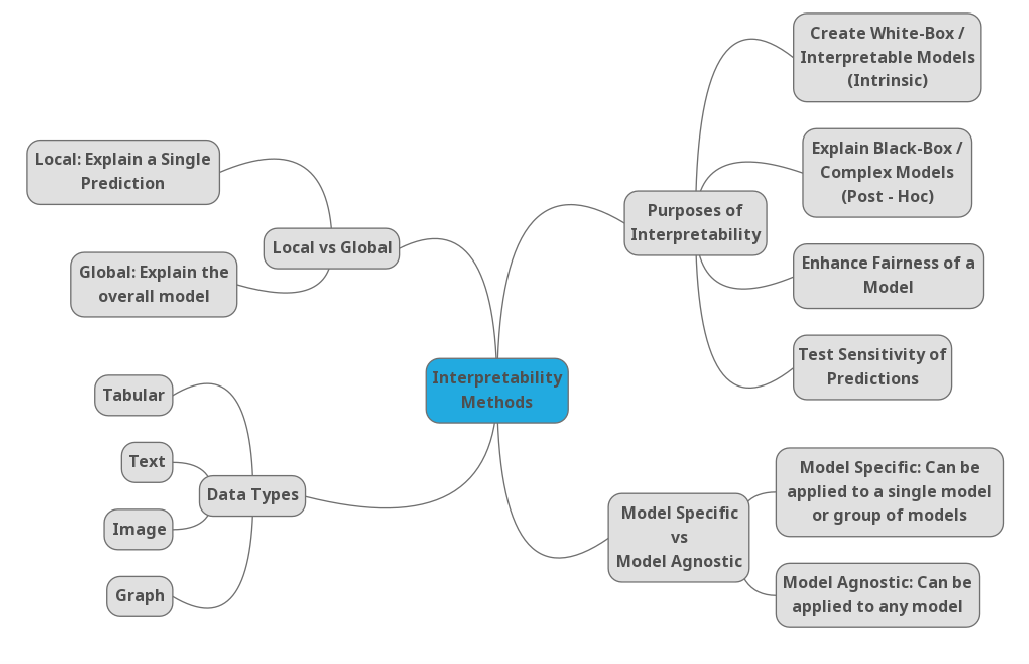
\includegraphics[height=2in]{images/explainability_taxonomies.png}
\caption{Taxonomies of Explainable AI techniques. Image taken from \cite{linardatos2021}}
\label{f:explainability_taxonomies}
\end{figure}

One such classification is based on model-agnostic (which can be applied to any model) versus model-dependent where the approach depends on the specific prediction algorithms used by the model.
The early works on this includes the use of explanation vectors introduced by David Baehrens et.al. in their paper \cite{baehrens2010explain}.
Local Interpretable Model-Agnostic Explanations (LIME) \cite{ribeiro2016should} is one of the most widely used tools to explain the predictions of any machine learning model.
LIME works by approximating the model behaviour locally by a simple interpretable surrogate model like linear model or decision tree. The approximation is restricted to a small local change in the input. As this technique looks only at the input and output of the model, this technique can be applied to any machine learning models.
However, the main drawback of the approach is that the surrogate model is only a local approximation and fails to capture the global behaviour.
Rabold et. al. in their recent work \cite{rabold2019enriching} builds on top of LIME and suggests an approach where classifiers' decisions can be explained in terms of logic rules. Their approach is unique in the sense that the predictions can be explained using relationships of objects within the image, whereas in most other approaches the decision is based on presence or absence of certain features.

Another famous technique called Layer-wise Relevance Propagation was introduced by Bach et.al. \cite{bach2015pixel} where the classifier decision is  back propagated and a relevance score is computed at each of the layers backwards until the input units are assigned a relevance score.
The work by Wojciech Samek et.al. \cite{samek2016evaluating} provides a quantitative  evaluation of Layer-wise Relevance Propagation and  suggests it as a better model as opposed to sensitivity based methods.

Scott et.al. introduced a unified approach for explainability which combines multiple methods and brings in a new class of additive feature importance measure (called SHapley) \cite{lundberg2017unified}.
Their method, known as SHapley Additive ExPlanations (SHAP) considers all  the interactions between features and provides an average measure of importance for each feature.

Another class of widely used algorithms for  Convolutional Neural Networks  targets at finding and highlighting the  regions in the input image that is responsible for the prediction.
These techniques, originally introduced in paper \cite{zhou2016learning}, generate a heatmap called Class Activation Map that will highlight the most sensitive regions in the input image.
Saliency Map, introduced by Symonyan et.al. in 2014 \cite{simonyan2014deep} is another variant of class activation map computed by optimizing the input image using the gradient of output prediction with respect to the input image.


Another criteria for classifying XAI techniques is based on the data type used like text, images, structured data (a specific case of which is tabular data) graph etc.
TODO add some example cases

Another criteria for classifying XAI techniques is based on the data type used like text, images, structured data (a specific case of which is tabular data) graph etc.

Yet another way of classifying explainability approach is based on whether the technique is applicable for individual instance or for the whole model.
TODO add some examples

\subsection{Concept Learning}
\subsection{Semi-supervised Learning}

\section{{ PROPOSED METHOD}}\label{proposed_method}

\subsection{Overview of Approach}
We start with a completely unlabelled dataset and solve a task like image classification or segmentation on this dataset by generating concepts and operators required to solve the task at hand.
However, the proposed approach is not completely unsupervised.
Instead, we propose an iterative algorithm where human feedback is taken interactively and the model is improved based on the feedback.
In this respect our approach is comparable to semi-supervised learning and active learning (write differences. active learning the goal is only to minimize manual annotation where as here there is an additional goal of adding explainability and also generalizing the learned concepts)

The proposed approach modifies the training procedure of deep learning models so that the model not only learns to perform the specific task,  but also learns a set of \textbf{generic modularized concepts} and \textbf{composition rules or operators} with the following objectives:
\begin{itemize}
\item The models final prediction can be explained using the concepts and operators learned.
\item A task like image classification or segmentation, which is solved using supervised methods today, can be solved in semi-supervised fashion requiring very less annotated samples.
\item We anticipate to accelerate the training process as the concepts are learned prior to ( or while) learning the final classification task.
\item The learned concepts can be used for other related task. This is in contrast with current transfer learning approaches where the model parameters that is being shared across tasks need not the modularized
\end{itemize}

Figure \ref{f:cnn_arch} shows the architecture of the proposed model used for the MNIST dataset.
For other more complex datasets, the overall structure remains the same except that more number of layers were added in encoder and decoder along with Batch Normalization \cite{ioffe2015} and regularization.
For MNIST, we use a variational autoencoder (VAE) with five layers of convolutional layers in the encoder and five layers of deconvolution layers in the decoder.
All layers, including the middle layer that generates the latent images, are fully convolutional.
We replaced the middle dense layer of in VAE, with a convolutional layer in order to create a latent image (as opposed to a one dimensional latent vector) that preserves the spatial relationship.
We added an additional loss component at the hidden layer 3 of the decoder in order to force this layer to learn the primitive visual concepts of the dataset.
The final layer of the decoder has sigmoid activation function and we use binary cross entropy loss as the MNIST images can be treated as binary images.

\begin{figure}
\centering
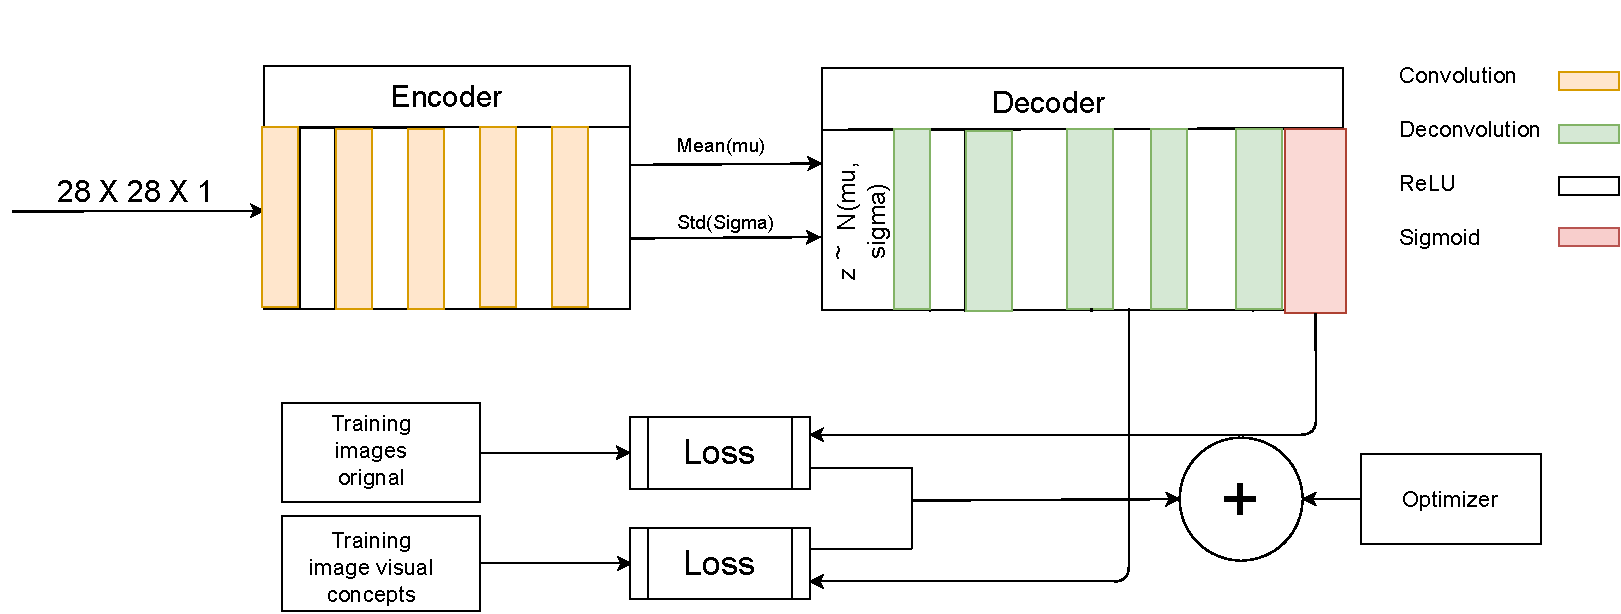
\includegraphics[height=2in]{images/cnn_arch}
\caption{Architecture of the proposed model for MNIST dataset. An additional loss component were added at layer 3 of decoder in Variational Autoencoder.
}
\label{f:cnn_arch}
\end{figure}

\subsection{Datasets}
The proposed approach is demonstrated on datasets of increasing complexity starting from MNIST, CIFAR-10, CIFAR-100, Marmot \cite{fang2012} dataset for table detection.
For adding the concept loss, the MNIST training set was first augmented by adding 3000 training images for each of the 18 concepts shown in Figure \ref{f:visual_concept}.
Some of the similar looking concepts in Figure \ref{f:visual_concept}, like the horizontal line segments and vertical line segments, were combined into one group to form 18 unique  visual concepts.
The steps for generating concepts are detailed in the sections below.

\subsection{Primary Visual Concepts}
Generating Visual Concepts
We augment the training set using images of randomly generated segments from MNIST images.
For each of the visual concepts shown in Figure \ref{f:visual_concept}, 3000 images were generated by randomly sampling the height, width and location of the segment from a normal distribution.
For each concept, the mean value of the height, width and location is kept the same as in Figure \ref{f:visual_concept}.
The number of visual concepts and their corresponding distributions are hyper parameters that will vary from dataset to dataset.
To generate the segments for each concept, we sampled heights, widths and location of top left corner (represented by two distributions for  $x$ and $y$ coordinates) from the respective concept's distributions and generated slices from randomly chosen training images.
Standard deviation for all distributions were kept as 1 pixel in our experiments.

\begin{figure}
\centering
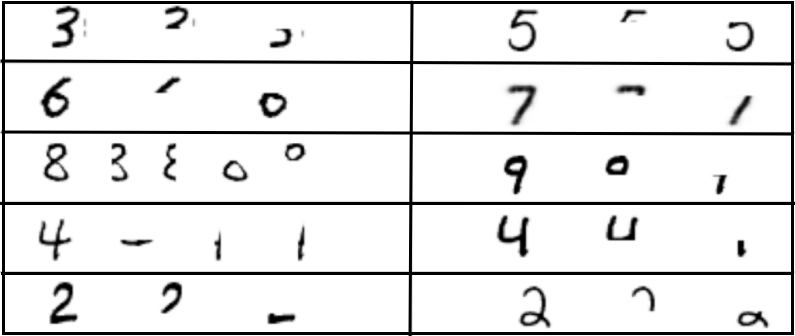
\includegraphics[height=2in]{images/visual_concepts.png}
\caption{Visual concepts generated from each of the digits in MNIST. Since there are two different types of images for digits 4 and 2 separate concepts were generated for each image. The width, height and location of these segments were used to define the mean value of a Normal distribution used for generating more samples.}
\label{f:visual_concept}
\end{figure}


\subsection{Composition of concepts}
\subsection{Network Architecture, Loss function and Training}

\section{Results and Discussion}\label{results_and_discussion}
\section{conclusion}\label{conclusion}
\section*{Acknowledgements}
The work of Q.H.C. is supported in part by the U.~S.~Dept.~of Energy
Grant No.~DE-AC02-06CH11357 and in part
by the Argonne National Lab.~and Univ.~of Chicago Joint Theory Institute
Grant No.~03921-07-137.
The work of S.K. and H.O. is supported in part by the Science and Technology
Development Fund (STDF) Project ID 437 and the ICTP Project ID 30.
The work of E.M. is supported in part by the U.~S.~Dept.~of Energy
Grant No. DE-FG03-94ER40837.


%\newpage
\bibliographystyle{unsrt}
\begin{thebibliography}{99}

\bibitem{jordan2015}
Jordan, Michael I., and Tom M. Mitchell. "Machine learning: Trends, perspectives, and prospects." Science 349.6245 (2015): 255-260.

% Explainability
\bibitem{ribeiro2016should} Ribeiro, Marco Tulio, Sameer Singh, and Carlos Guestrin. "" Why should i trust you?" Explaining the predictions of any classifier." Proceedings of the 22nd ACM SIGKDD international conference on knowledge discovery and data mining. 2016.
\bibitem{lundberg2017unified} Lundberg, Scott M., and Su-In Lee. "A unified approach to interpreting model predictions." Proceedings of the 31st international conference on neural information processing systems. 2017.
\bibitem{zhou2016learning}Zhou, Bolei, et al. "Learning deep features for discriminative localization." Proceedings of the IEEE conference on computer vision and pattern recognition. 2016.
\bibitem{baehrens2010explain} Baehrens, David, et al. "How to explain individual classification decisions." The Journal of Machine Learning Research 11 (2010): 1803-1831.
\bibitem{rabold2019enriching} Rabold, Johannes, et al. "Enriching Visual with Verbal Explanations for Relational Concepts--Combining LIME with Aleph." arXiv preprint arXiv:1910.01837 (2019).
\bibitem{bach2015pixel} Bach, Sebastian, et al. "On pixel-wise explanations for non-linear classifier decisions by layer-wise relevance propagation." PloS one 10.7 (2015): e0130140.
\bibitem{samek2016evaluating} Samek, Wojciech, et al. "Evaluating the visualization of what a deep neural network has learned." IEEE transactions on neural networks and learning systems 28.11 (2016): 2660-2673.
\bibitem{simonyan2014deep} Simonyan, Karen, Andrea Vedaldi, and Andrew Zisserman. "Deep inside convolutional networks: Visualising image classification models and saliency maps." arXiv preprint arXiv:1312.6034 (2013).
\bibitem{doshi2017} Doshi-Velez, Finale, and Been Kim. "Towards a rigorous science of interpretable machine learning." arXiv preprint arXiv:1702.08608 (2017).
\bibitem{linardatos2021} Linardatos, Pantelis, Vasilis Papastefanopoulos, and Sotiris Kotsiantis. "Explainable AI: A review of machine learning interpretability methods." Entropy 23.1 (2021): 18.
\bibitem{wu2021} Wu, Leihong, et al. "Trade-off Predictivity and Explainability for Machine-Learning Powered Predictive Toxicology: An in-Depth Investigation with Tox21 Data Sets." Chemical Research in Toxicology 34.2 (2021): 541-549.

% Datasets
\bibitem{fang2012}Fang, Jing, et al. "Dataset, ground-truth and performance metrics for table detection evaluation." 2012 10th IAPR International Workshop on Document Analysis Systems. IEEE, 2012.

% Concept Learning
\bibitem{lake2015} Lake, Brenden M., Ruslan Salakhutdinov, and Joshua B. Tenenbaum. "Human-level concept learning through probabilistic program induction." Science 350.6266 (2015): 1332-1338.
\bibitem{tenenbaum2019}Tenenbaum, Josh. Bayesian Program Learning and Concept Induction. Massachusetts Institute of Technology Cambridge United States, 2019.
\bibitem{nanayakkara2018} Nanayakkara, Shane, et al. "Characterising risk of in-hospital mortality following cardiac arrest using machine learning: A retrospective international registry study." PLoS medicine 15.11 (2018): e1002709.
\bibitem{miller2019} Tim Miller, Explanation in artificial intelligence: Insights from the social sciences, Artificial Intelligence, Volume 267,
2019, Pages 1-38,  ISSN 0004-3702, https://doi.org/10.1016/j.artint.2018.07.007. (https://www.sciencedirect.com/science/article/pii/S0004370218305988)

%autoencoder
\bibitem{kingma2013auto} Kingma, Diederik P., and Max Welling. "Auto-encoding variational bayes." arXiv preprint arXiv:1312.6114 (2013).

%DL techniques
\bibitem{ioffe2015} Ioffe, Sergey, and Christian Szegedy. "Batch normalization: Accelerating deep network training by reducing internal covariate shift." International conference on machine learning. PMLR, 2015.

\end{thebibliography}

\end{document}






